% Options for packages loaded elsewhere
\PassOptionsToPackage{unicode}{hyperref}
\PassOptionsToPackage{hyphens}{url}
\PassOptionsToPackage{dvipsnames,svgnames,x11names}{xcolor}
%
\documentclass[
  letterpaper,
  DIV=11,
  numbers=noendperiod]{scrreport}

\usepackage{amsmath,amssymb}
\usepackage{lmodern}
\usepackage{iftex}
\ifPDFTeX
  \usepackage[T1]{fontenc}
  \usepackage[utf8]{inputenc}
  \usepackage{textcomp} % provide euro and other symbols
\else % if luatex or xetex
  \usepackage{unicode-math}
  \defaultfontfeatures{Scale=MatchLowercase}
  \defaultfontfeatures[\rmfamily]{Ligatures=TeX,Scale=1}
\fi
% Use upquote if available, for straight quotes in verbatim environments
\IfFileExists{upquote.sty}{\usepackage{upquote}}{}
\IfFileExists{microtype.sty}{% use microtype if available
  \usepackage[]{microtype}
  \UseMicrotypeSet[protrusion]{basicmath} % disable protrusion for tt fonts
}{}
\makeatletter
\@ifundefined{KOMAClassName}{% if non-KOMA class
  \IfFileExists{parskip.sty}{%
    \usepackage{parskip}
  }{% else
    \setlength{\parindent}{0pt}
    \setlength{\parskip}{6pt plus 2pt minus 1pt}}
}{% if KOMA class
  \KOMAoptions{parskip=half}}
\makeatother
\usepackage{xcolor}
\setlength{\emergencystretch}{3em} % prevent overfull lines
\setcounter{secnumdepth}{5}
% Make \paragraph and \subparagraph free-standing
\ifx\paragraph\undefined\else
  \let\oldparagraph\paragraph
  \renewcommand{\paragraph}[1]{\oldparagraph{#1}\mbox{}}
\fi
\ifx\subparagraph\undefined\else
  \let\oldsubparagraph\subparagraph
  \renewcommand{\subparagraph}[1]{\oldsubparagraph{#1}\mbox{}}
\fi


\providecommand{\tightlist}{%
  \setlength{\itemsep}{0pt}\setlength{\parskip}{0pt}}\usepackage{longtable,booktabs,array}
\usepackage{calc} % for calculating minipage widths
% Correct order of tables after \paragraph or \subparagraph
\usepackage{etoolbox}
\makeatletter
\patchcmd\longtable{\par}{\if@noskipsec\mbox{}\fi\par}{}{}
\makeatother
% Allow footnotes in longtable head/foot
\IfFileExists{footnotehyper.sty}{\usepackage{footnotehyper}}{\usepackage{footnote}}
\makesavenoteenv{longtable}
\usepackage{graphicx}
\makeatletter
\def\maxwidth{\ifdim\Gin@nat@width>\linewidth\linewidth\else\Gin@nat@width\fi}
\def\maxheight{\ifdim\Gin@nat@height>\textheight\textheight\else\Gin@nat@height\fi}
\makeatother
% Scale images if necessary, so that they will not overflow the page
% margins by default, and it is still possible to overwrite the defaults
% using explicit options in \includegraphics[width, height, ...]{}
\setkeys{Gin}{width=\maxwidth,height=\maxheight,keepaspectratio}
% Set default figure placement to htbp
\makeatletter
\def\fps@figure{htbp}
\makeatother

\KOMAoption{captions}{tableheading}
\makeatletter
\@ifpackageloaded{tcolorbox}{}{\usepackage[many]{tcolorbox}}
\@ifpackageloaded{fontawesome5}{}{\usepackage{fontawesome5}}
\definecolor{quarto-callout-color}{HTML}{909090}
\definecolor{quarto-callout-note-color}{HTML}{0758E5}
\definecolor{quarto-callout-important-color}{HTML}{CC1914}
\definecolor{quarto-callout-warning-color}{HTML}{EB9113}
\definecolor{quarto-callout-tip-color}{HTML}{00A047}
\definecolor{quarto-callout-caution-color}{HTML}{FC5300}
\definecolor{quarto-callout-color-frame}{HTML}{acacac}
\definecolor{quarto-callout-note-color-frame}{HTML}{4582ec}
\definecolor{quarto-callout-important-color-frame}{HTML}{d9534f}
\definecolor{quarto-callout-warning-color-frame}{HTML}{f0ad4e}
\definecolor{quarto-callout-tip-color-frame}{HTML}{02b875}
\definecolor{quarto-callout-caution-color-frame}{HTML}{fd7e14}
\makeatother
\makeatletter
\makeatother
\makeatletter
\@ifpackageloaded{bookmark}{}{\usepackage{bookmark}}
\makeatother
\makeatletter
\@ifpackageloaded{caption}{}{\usepackage{caption}}
\AtBeginDocument{%
\ifdefined\contentsname
  \renewcommand*\contentsname{Table of contents}
\else
  \newcommand\contentsname{Table of contents}
\fi
\ifdefined\listfigurename
  \renewcommand*\listfigurename{List of Figures}
\else
  \newcommand\listfigurename{List of Figures}
\fi
\ifdefined\listtablename
  \renewcommand*\listtablename{List of Tables}
\else
  \newcommand\listtablename{List of Tables}
\fi
\ifdefined\figurename
  \renewcommand*\figurename{Figure}
\else
  \newcommand\figurename{Figure}
\fi
\ifdefined\tablename
  \renewcommand*\tablename{Table}
\else
  \newcommand\tablename{Table}
\fi
}
\@ifpackageloaded{float}{}{\usepackage{float}}
\floatstyle{ruled}
\@ifundefined{c@chapter}{\newfloat{codelisting}{h}{lop}}{\newfloat{codelisting}{h}{lop}[chapter]}
\floatname{codelisting}{Listing}
\newcommand*\listoflistings{\listof{codelisting}{List of Listings}}
\makeatother
\makeatletter
\@ifpackageloaded{caption}{}{\usepackage{caption}}
\@ifpackageloaded{subcaption}{}{\usepackage{subcaption}}
\makeatother
\makeatletter
\@ifpackageloaded{tcolorbox}{}{\usepackage[many]{tcolorbox}}
\makeatother
\makeatletter
\@ifundefined{shadecolor}{\definecolor{shadecolor}{rgb}{.97, .97, .97}}
\makeatother
\makeatletter
\makeatother
\ifLuaTeX
  \usepackage{selnolig}  % disable illegal ligatures
\fi
\IfFileExists{bookmark.sty}{\usepackage{bookmark}}{\usepackage{hyperref}}
\IfFileExists{xurl.sty}{\usepackage{xurl}}{} % add URL line breaks if available
\urlstyle{same} % disable monospaced font for URLs
\hypersetup{
  pdftitle={CRIMES DE TRÂNSITO},
  pdfauthor={Mário Diego Rocha Valente},
  colorlinks=true,
  linkcolor={blue},
  filecolor={Maroon},
  citecolor={Blue},
  urlcolor={Blue},
  pdfcreator={LaTeX via pandoc}}

\title{\textbf{CRIMES DE TRÂNSITO}}
\usepackage{etoolbox}
\makeatletter
\providecommand{\subtitle}[1]{% add subtitle to \maketitle
  \apptocmd{\@title}{\par {\large #1 \par}}{}{}
}
\makeatother
\subtitle{\textbf{Conceitos Fundamentais}}
\author{\textbf{Mário Diego Rocha Valente}}
\date{2/28/24}

\begin{document}
\maketitle
\ifdefined\Shaded\renewenvironment{Shaded}{\begin{tcolorbox}[boxrule=0pt, enhanced, interior hidden, borderline west={3pt}{0pt}{shadecolor}, breakable, sharp corners, frame hidden]}{\end{tcolorbox}}\fi

\renewcommand*\contentsname{Table of contents}
{
\hypersetup{linkcolor=}
\setcounter{tocdepth}{2}
\tableofcontents
}
\bookmarksetup{startatroot}

\hypertarget{prefuxe1cio}{%
\chapter*{Prefácio}\label{prefuxe1cio}}
\addcontentsline{toc}{chapter}{Prefácio}

\markboth{Prefácio}{Prefácio}

O número crescente de ações penais e cíveis oriundas de enetos de
trânsito, desde processos contra o ente público fiscalizador do
trânsito., ações indenizatórias, defesas penais, ações coletivas
fundadas no direito de trânsito, demostram par aqualquer operador do
direito a importância dessa temática jurídica.

Indispensável é a formulação de políticas públicas permanentes de
educação no trânsito para redução de sinistros, com objetivos e
responsabilidades bem claramente definidos, especialmente quanto aos
sinistros envolvendo motocicletas, os quais representam quase um um
terço das mortes.

\bookmarksetup{startatroot}

\hypertarget{conceitos-fundamentais}{%
\chapter{Conceitos Fundamentais}\label{conceitos-fundamentais}}

\hypertarget{leis}{%
\section{Leis}\label{leis}}

No seu sentido mais amplo, o termo ``lei'' significa sempre ordenação
através de regularidades. Todo condutor tem a obrigação de conhecer as
leis de trânsito, o dever social de cumpri-las, e estará sujeito a
multas e penalidades toda vez que transgredi-las.

\begin{longtable}[]{@{}
  >{\centering\arraybackslash}p{(\columnwidth - 2\tabcolsep) * \real{0.4722}}
  >{\centering\arraybackslash}p{(\columnwidth - 2\tabcolsep) * \real{0.5278}}@{}}
\toprule()
\endhead
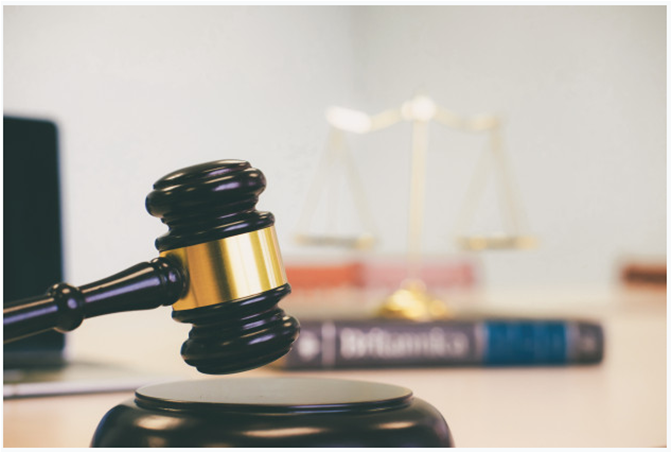
\includegraphics{./images/image-2035638006.png} &
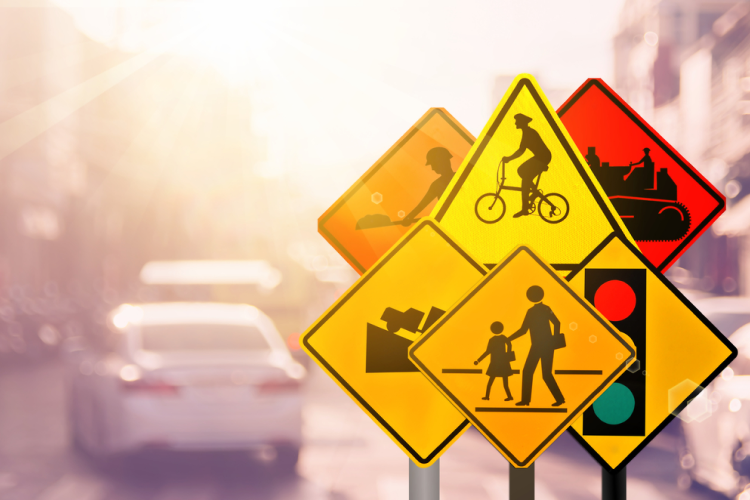
\includegraphics[width=3.52083in,height=\textheight]{./images/lei1-02.png} \\
\bottomrule()
\end{longtable}

\hypertarget{truxe2nsito}{%
\section{Trânsito}\label{truxe2nsito}}

1º Considera-se trânsito a utilização das vias por pessoas, veículos e
animais, isolados ou em grupos, CONDUZIDOS OU NÃO, para fins de
circulação, parada, estacionamento e operação de carga ou descarga.

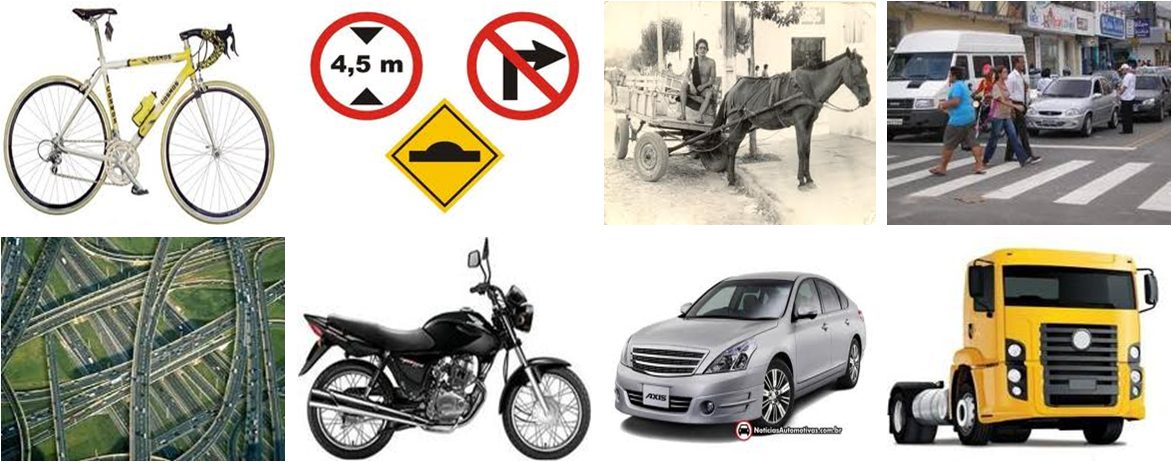
\includegraphics{./images/image-1961589352.png}

\hypertarget{direuxe7uxe3o-defensiva}{%
\section{Direção Defensiva}\label{direuxe7uxe3o-defensiva}}

Dirigir Defensivamente(português brasileiro) OU Condução
Defensiva(português europeu) é o conjunto de medidas e procedimentos
utilizados para prever ou minimizar as consequências dos acidentes de
trânsito.

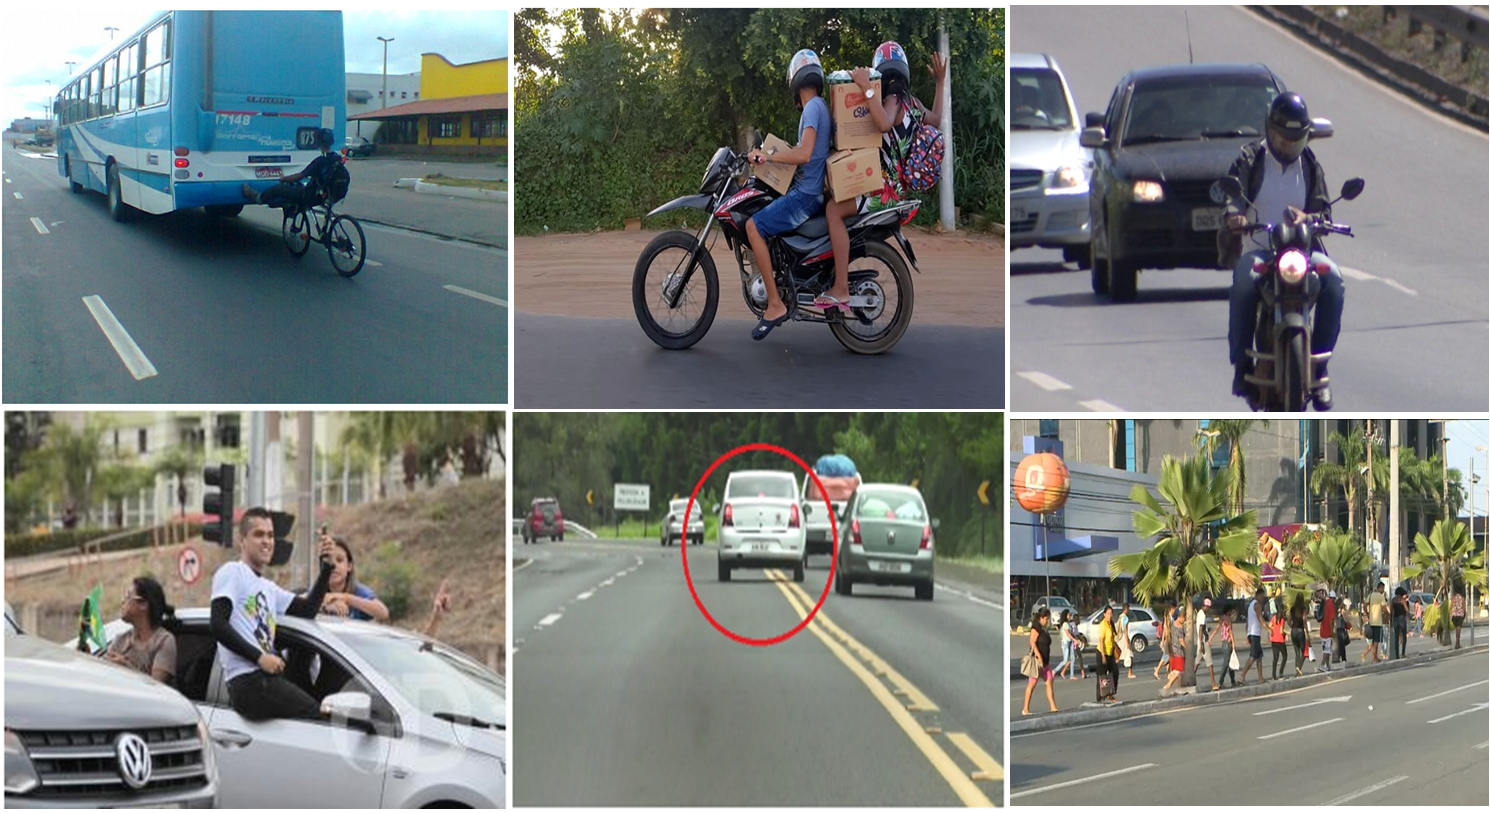
\includegraphics{./images/image-1151365635.png}

Baseado na noção de que em todo acidente sempre está presente uma falha
humana relacionada ou a negligência, ou imprudência, ou imperícia, a
direção defensiva pretende que o motorista que a emprega seja um
elemento ativo na alteração ou eliminação dos fatores que possam vir a
causar acidentes.

Além disso, ao longo da vida, acontecem as mais variadas circunstâncias
de risco, devidas ao Ambiente e aos Outros Condutores;

Desse modo, o motorista profissional precisa conhecer as Manobras
Defensivas que o ajudam a diminuir o risco de acidentes e a preservar
sua vida, a vida dos outros condutores, o veículo e os passageiros;

\hypertarget{negliguxeancia}{%
\subsection{\texorpdfstring{\textbf{Negligência}}{Negligência}}\label{negliguxeancia}}

A negligência pode ser definida como descaso, displicência ou desleixo.
Muitos sinistros e mortes são causados por negligência.

\hypertarget{impruduxeancia}{%
\subsection{\texorpdfstring{\textbf{Imprudência}}{Imprudência}}\label{impruduxeancia}}

A imprudência, elemento de presença constante no trânsito brasileiro, o
motorista imprudente é aquele que pratica uma ação desconsiderando os
riscos causados por ela.

\hypertarget{imperuxedcia}{%
\subsection{\texorpdfstring{\textbf{Imperícia}}{Imperícia}}\label{imperuxedcia}}

A imperícia ou a falta de habilidade é uma importante causa de
sinistros. Geralmente é proveniente de má formação ou treinamento
inadequado do condutor.

\hypertarget{crimes}{%
\section{Crimes}\label{crimes}}

É necessário que se faça, a distinção entre crimes de trânsito, crimes
em trânsito e crimes no trânsito.

\hypertarget{crimes-de-truxe2nsito}{%
\subsubsection{\texorpdfstring{Crimes \textbf{DE}
Trânsito}{Crimes DE Trânsito}}\label{crimes-de-truxe2nsito}}

Os crimes de trânsito são aqueles que se ecnontram expressamente
previsto no CTB (na Seção II do Capítulo XIX, intitulada ``Dos Crimes em
Espécie'', indo ao art. 302 ao art. 312, consoante já mensionado).

\hypertarget{crimes-em-truxe2nsito}{%
\subsection{\texorpdfstring{Crimes \textbf{EM}
Trânsito}{Crimes EM Trânsito}}\label{crimes-em-truxe2nsito}}

Os crime em trânsito, por sua vez, envolvem mais de dois países, sendo
clássico o exemplo do tráfico internacional de drogas.

\hypertarget{crimes-no-truxe2nsito}{%
\subsection{\texorpdfstring{Crimes \textbf{NO}
Trânsito}{Crimes NO Trânsito}}\label{crimes-no-truxe2nsito}}

A expressão crimes no trânsito pode se materializar a partir de ínumeras
situações, haja vista ter por base unicamente o espaço no qual a conduta
delituosa - ação ou omissão - é praticada, sendo exemplos desde o crime
de uso de documento falso (art. 304 c.c o art. 297, caput, do Código
Penal), o crime de roubo (art. 157 do Código Penal) perpetrado no
trânsito.

\begin{longtable}[]{@{}
  >{\centering\arraybackslash}p{(\columnwidth - 4\tabcolsep) * \real{0.3333}}
  >{\centering\arraybackslash}p{(\columnwidth - 4\tabcolsep) * \real{0.3333}}
  >{\centering\arraybackslash}p{(\columnwidth - 4\tabcolsep) * \real{0.3333}}@{}}
\toprule()
\endhead

\includegraphics{./images/crime1-01.jpg} &
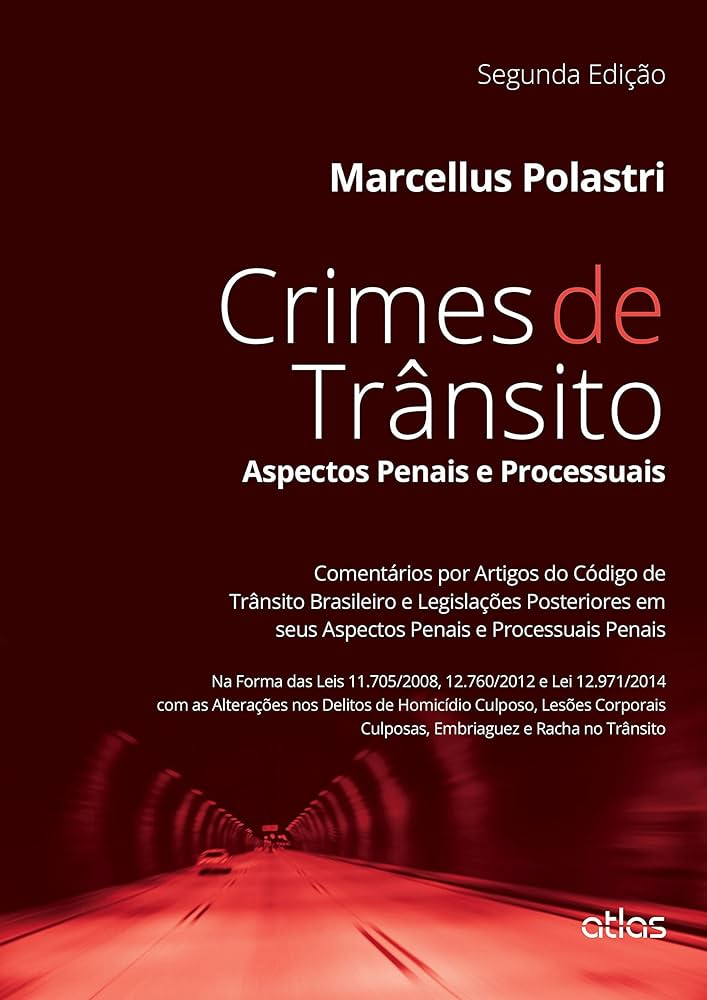
\includegraphics{./images/crime3-01.jpg} &
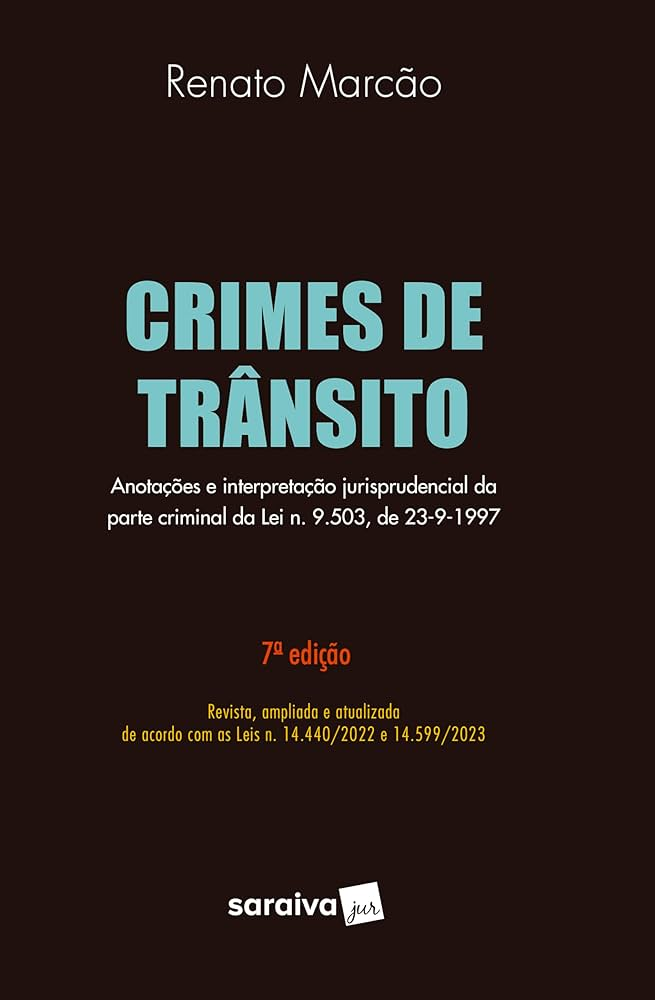
\includegraphics[width=2.16667in,height=\textheight]{./images/crime2-01.jpg} \\
\bottomrule()
\end{longtable}

\hypertarget{lei-nuxba-9.0991995}{%
\section{\texorpdfstring{\textbf{Lei Nº
9.099/1995}}{Lei Nº 9.099/1995}}\label{lei-nuxba-9.0991995}}

Com relação a Lei Nº 9.099/1995, este diploma institui os
\textbf{Juizados Especiais Cíveis e Criminais na Justiça Estadual}.

\begin{longtable}[]{@{}
  >{\centering\arraybackslash}p{(\columnwidth - 4\tabcolsep) * \real{0.3333}}
  >{\centering\arraybackslash}p{(\columnwidth - 4\tabcolsep) * \real{0.3333}}
  >{\centering\arraybackslash}p{(\columnwidth - 4\tabcolsep) * \real{0.3333}}@{}}
\toprule()
\endhead
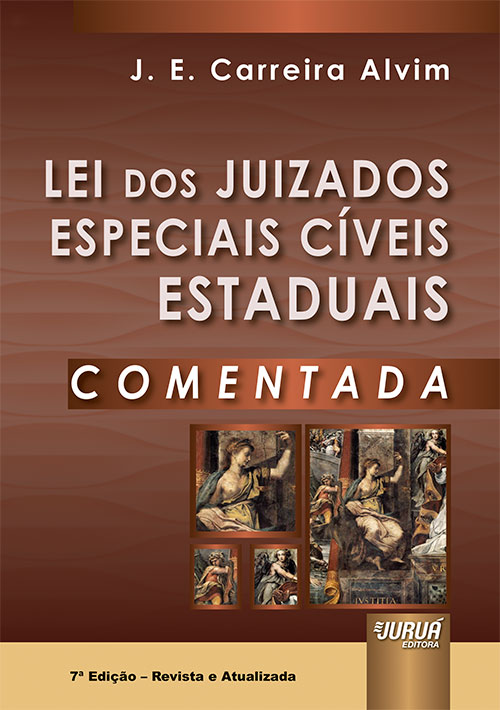
\includegraphics{./images/juizado1-01.jpg} &
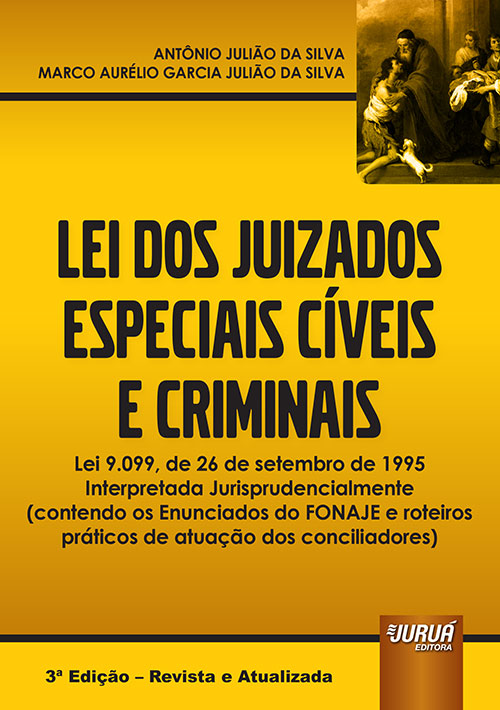
\includegraphics{./images/juizado3-01.jpg} &

\includegraphics{./images/juizado2-01.jpg} \\
\bottomrule()
\end{longtable}

No que tange especificamente ao Juizado Especial Criminal (JECrim), tal
órgão tem competência, para a concialiação, o julgamento e a execução
das infrações de menor potencial ofensivo, nor termos do \textbf{art.
60} da menionada lei.

Por definição legal, consideram-se infrações penais de menor potencial
ofensivo as contravenções penais e os crimes a que a lei comine pena
máxima não superior a dois anos., cumula ou não com multa (art. 61, Lei
9.099/1995). Essas infrações seguem um procedimento diferente daquele
previsto no Código de Processo Penal, procedimento esse repleto de
medidas despenalizadoras, como a \textbf{Transação Penal} e a
\textbf{Composição Civil}, que representam parcial renúncia ao direito
de punir do Estado.

Dos crimes previsto pelo Código de Trânsito, apenas o Homicídio Culposo
na direção veículo automotor (\textbf{art. 302}), a condução do veículo
automotor com capacidade psicomotora alterada (\textbf{art. 306}) e a
participação em corrida, disputa ou competição automobilística não
autorizada pela autoridade competente (\textbf{art. 308}) têm pena
máxima superior a dois anos, pelo que ficam excluídos da aplicação da
Lei nº 9.099/1995.

No âmbito federal, os Juizados Especiais são regulados pela \textbf{Lei
nº 10.259/2001}.

\bookmarksetup{startatroot}

\hypertarget{disposiuxe7uxf5es-gerais}{%
\chapter{Disposições Gerais}\label{disposiuxe7uxf5es-gerais}}

\hypertarget{introduuxe7uxe3o}{%
\section{Introdução}\label{introduuxe7uxe3o}}

Os crimes cometidos na direção de veículos automotores, em sua grande
maioria, estão tipificados no \textbf{Capítulo XIX} do Código de
Trânsito Brasileiro (CTB), entre os arts. 302 e 312. O legislador
tratou, desde logo, de limitar o ambito de alcance do CTB, estabelecendo
que o Código regula apenas os crimes cometidos na direção de veículo
automotor.

Deste modo, \textbf{Não} se aplicam as normas do Código de Trânsito a
fatos criminosos praticados na direção veículos de propução humana, com
a bicicleta, bem como aqueles cometidos na direção de veículos de tração
animal, com a carroça.

Tratando-se de crime cometido na direção de veículo automotor,
aplicar-se-ão primeiramente as regras do Código de Trânsito, por ser
\textbf{Norma Especial}.

Assim, no que não for incompatível com a legislação de trânsito, bem
como em caso de omissões, são aplicável com a legislação de trânsito,
bem como em caso de omissões, são aplicáveis as normas gerais do
\textbf{Código Penal} e do \textbf{Código de Processo Penal}.

Porém, isto não implica dizer que não se pode cometer crimes previstos
no Código Penal ou Contravenções previstas na \textbf{Lei de
Contravenções Penais} quando se está na direção de veículo automotor,
devendo a análise da tipificação penal ocorrer à luz do \textbf{Caso
Concreto}.

\hypertarget{artigo-291---ctb}{%
\section{\texorpdfstring{\textbf{Artigo 291 -
CTB}}{Artigo 291 - CTB}}\label{artigo-291---ctb}}

\begin{tcolorbox}[enhanced jigsaw, titlerule=0mm, colframe=quarto-callout-important-color-frame, opacityback=0, breakable, colbacktitle=quarto-callout-important-color!10!white, left=2mm, bottomtitle=1mm, toprule=.15mm, rightrule=.15mm, arc=.35mm, leftrule=.75mm, bottomrule=.15mm, opacitybacktitle=0.6, toptitle=1mm, title=\textcolor{quarto-callout-important-color}{\faExclamation}\hspace{0.5em}{Important}, colback=white, coltitle=black]

``\textbf{Aos crimes cometidos na direção de veículos automotores,
previstos neste Código, aplicam-se as normas gerais do Código Penal e do
Código de Processo Penal, se este Capítulo não dispuser de modo diverso,
bem como a Lei nº 9.099, de 26 de setembro de 1995, no que couber}''.

\end{tcolorbox}

\hypertarget{uxba}{%
\subsection{\texorpdfstring{\textbf{§ 1º}}{§ 1º}}\label{uxba}}

Aplica-se aos crimes de trânsito de lesão corporal culposa o disposto
nos arts. 74, 76 e 88 da Lei no 9.099, de 26 de setembro de 1995, exceto
se o agente estiver: (Renumerado do parágrafo único pela Lei nº 11.705,
de 2008)

\begin{itemize}
\item
  \textbf{I} - sob a influência de álcool ou qualquer outra substância
  psicoativa que determine dependência; (Incluído pela Lei nº 11.705, de
  2008)
\item
  \textbf{II} - participando, em via pública, de corrida, disputa ou
  competição automobilística, de exibição ou demonstração de perícia em
  manobra de veículo automotor, não autorizada pela autoridade
  competente; (Incluído pela Lei nº 11.705, de 2008)
\item
  \textbf{III} - transitando em velocidade superior à máxima permitida
  para a via em 50 km/h (cinqüenta quilômetros por hora). (Incluído pela
  Lei nº 11.705, de 2008)
\end{itemize}

Este parágrafo, com as alterações produzidas pela Lei 11.705/2008
modifica significativamente a aplicabilidade da Lei 9.099/1995 em
relação aos Crimes de Trânsito cometidos na direção de veículo
automotor. Especificamente ao delito tipificado no art. 303 do Código,
lesão corporal culposa no trânsito, embora se trate de uma infraçãp
penal de menor potencial ofensivo, os três artigos citados (74,76 e 88),
que prevem, respectivamente, a composição civil, a transação penal e a
necessidade de representação para propositura da ação penal, deixarão de
ser aplicados em benefício do autor, quando este se encontrar em uma das
circunstâncias definidas neste dispositivo.

Desta forma, temos que o delito do art. 303, embora continue a ser um
crime de menor potencial ofensivo, por sua pena máxima não exceder a
dois anos, não atrairá a aplicação dos benefícios mensionados se o
agente estiver em uma das três situações:

\begin{itemize}
\tightlist
\item
  \textbf{Sob a Influência de Alcool ou qualquer outra substância
  psicoativa que determine dependência};
\item
  \textbf{Participando, em via pública, de corrida, disputa ou
  competição automobilística, de exibição ou demonstração de perícia em
  manobra de veículo automotor, não autorizada pela autoridade
  competente};
\item
  \textbf{Transitando em velocidade superior à máxima permitida para a
  via em 50km/h}
\end{itemize}

Frise-se, desde logo, que, em se verificar a situação prevista noinc. I
deste dispositivo, a lesão corporal culposa praticada na direção de
veículo automotor será tida como \textbf{Qualificada} e, por
conseguinte, será punida de modo mais severo, conforme alteração
promovida pela lei 13.546/2017, a qual acrescentou um novo parágrafo ao
art.303 do CTB.

Trata-se, portanto, de uma norma de exceção, que afasta a incidência da
regra geral. Dentre as hipóteses citadas, a mais observada nas vias
públicas, infelizmente, é a condução de veículo sob a influência de
álcool ou sibstância análoga. Nesses casos, os tribunais pátrios,
corretamente, vêm entendendo trata-se de Ação Penal Pública
Incondicionada, sendo desnecessária a representação da vítima.

\hypertarget{uxba-1}{%
\subsection{\texorpdfstring{\textbf{§ 2º}}{§ 2º}}\label{uxba-1}}

Nas hipóteses previstas no § 1o deste artigo, deverá ser instaurado
inquérito policial para a investigação da infração penal. (Incluído pela
Lei nº 11.705, de 2008)

Conforme já mensinado, os crimes capitulados como de menor potencial
ofensivo observam procedimento

\hypertarget{uxba-2}{%
\subsection{\texorpdfstring{\textbf{§ 3º}}{§ 3º}}\label{uxba-2}}

(VETADO). (Incluído pela Lei nº 13.546, de 2017)

\hypertarget{uxba-3}{%
\subsection{\texorpdfstring{\textbf{§ 4º}}{§ 4º}}\label{uxba-3}}

O juiz fixará a pena-base segundo as diretrizes previstas no art. 59 do
Decreto-Lei nº 2.848, de 7 de dezembro de 1940 (Código Penal), dando
especial atenção à culpabilidade do agente e às circunstâncias e
consequências do crime. (Incluído pela Lei nº 13.546, de 2017)

\hypertarget{artigo-292---ctb}{%
\section{\texorpdfstring{\textbf{Artigo 292 -
CTB}}{Artigo 292 - CTB}}\label{artigo-292---ctb}}

\begin{tcolorbox}[enhanced jigsaw, titlerule=0mm, colframe=quarto-callout-important-color-frame, opacityback=0, breakable, colbacktitle=quarto-callout-important-color!10!white, left=2mm, bottomtitle=1mm, toprule=.15mm, rightrule=.15mm, arc=.35mm, leftrule=.75mm, bottomrule=.15mm, opacitybacktitle=0.6, toptitle=1mm, title=\textcolor{quarto-callout-important-color}{\faExclamation}\hspace{0.5em}{Important}, colback=white, coltitle=black]

\textbf{``A suspensão ou a proibição de se obter a permissão ou a
habilitação para dirigir veículo automotor pode ser imposta isolada ou
cumulativamente com outras penalidades. (Redação dada pela Lei nº
12.971, de 2014)''}

\end{tcolorbox}

A penalidade de suspensão ou proibição de se obter a permissão ou a
habilitação para dirigir veículo automotor não se confunde com a
penalidade aplicada pela \textbf{Autoridade de Trânsito}, prevista nos
arts. 256, III, e 261 do CTB, que tem natureza administrativa. A sanção
prevista neste artigo é aplicada pela \textbf{Autoridade Judiciária},
apartir do cometimento de crimes de trânsito, tendo, pois, natureza
Criminal.

Cabe observar que o artigo dis respeito a duas situações. Na primeira, o
juiz aplica a penalidade de suspensão do direito de dirigir em relação a
uma pessoa que já devidamente habilitada para conduzir veéiculos
automotores em vias públicas; na segunda, a autoridade judiciária aplica
a penalidade de proibição de se obter a permissão ou a habilitação para
dirigir veículos automotores em vias publicas em relação a uma pessoa
que ainda \textbf{Não} esteja devidamente habilitada, nos termos do CTB.

Essa pessoa poderá, inclusive, já ter se inscrito do DETRAN, com a
abertura do RENACH (Registro Nacional de Carteiras de Habilitação), e
estar em processo de aprendizagem, mas, em razão de ter cometido
determinado crime de trânsito, \textbf{o juiz poderá lhe aplicar pena
impeditiva de obter sua habilitação}, por determinado período de tempo,
que varia de dois meses a cinco anos, nos termos do artigo seguinte.

\hypertarget{artigo-293---ctb}{%
\section{\texorpdfstring{\textbf{Artigo 293 -
CTB}}{Artigo 293 - CTB}}\label{artigo-293---ctb}}

\begin{tcolorbox}[enhanced jigsaw, titlerule=0mm, colframe=quarto-callout-important-color-frame, opacityback=0, breakable, colbacktitle=quarto-callout-important-color!10!white, left=2mm, bottomtitle=1mm, toprule=.15mm, rightrule=.15mm, arc=.35mm, leftrule=.75mm, bottomrule=.15mm, opacitybacktitle=0.6, toptitle=1mm, title=\textcolor{quarto-callout-important-color}{\faExclamation}\hspace{0.5em}{Important}, colback=white, coltitle=black]

\textbf{``A penalidade de suspensão ou de proibição de se obter a
permissão ou a habilitação, para dirigir veículo automotor, tem a
duração de dois meses a cinco anos.''}

\end{tcolorbox}

\hypertarget{artigo-294---ctb}{%
\section{\texorpdfstring{\textbf{Artigo 294 -
CTB}}{Artigo 294 - CTB}}\label{artigo-294---ctb}}

\begin{tcolorbox}[enhanced jigsaw, titlerule=0mm, colframe=quarto-callout-important-color-frame, opacityback=0, breakable, colbacktitle=quarto-callout-important-color!10!white, left=2mm, bottomtitle=1mm, toprule=.15mm, rightrule=.15mm, arc=.35mm, leftrule=.75mm, bottomrule=.15mm, opacitybacktitle=0.6, toptitle=1mm, title=\textcolor{quarto-callout-important-color}{\faExclamation}\hspace{0.5em}{Important}, colback=white, coltitle=black]

\textbf{Em qualquer fase da investigação ou da ação penal, havendo
necessidade para a garantia da ordem pública, poderá o juiz, como medida
cautelar, de ofício, ou a requerimento do Ministério Público ou ainda
mediante representação da autoridade policial, decretar, em decisão
motivada, a suspensão da permissão ou da habilitação para dirigir
veículo automotor, ou a proibição de sua obtenção.}

\textbf{Parágrafo único. Da decisão que decretar a suspensão ou a medida
cautelar, ou da que indeferir o requerimento do Ministério Público,
caberá recurso em sentido estrito, sem efeito suspensivo.}

\end{tcolorbox}

\hypertarget{artigo-295---ctb}{%
\section{\texorpdfstring{\textbf{Artigo 295 -
CTB}}{Artigo 295 - CTB}}\label{artigo-295---ctb}}

\begin{tcolorbox}[enhanced jigsaw, titlerule=0mm, colframe=quarto-callout-important-color-frame, opacityback=0, breakable, colbacktitle=quarto-callout-important-color!10!white, left=2mm, bottomtitle=1mm, toprule=.15mm, rightrule=.15mm, arc=.35mm, leftrule=.75mm, bottomrule=.15mm, opacitybacktitle=0.6, toptitle=1mm, title=\textcolor{quarto-callout-important-color}{\faExclamation}\hspace{0.5em}{Important}, colback=white, coltitle=black]

\textbf{``A suspensão para dirigir veículo automotor ou a proibição de
se obter a permissão ou a habilitação será sempre comunicada pela
autoridade judiciária ao Conselho Nacional de Trânsito - CONTRAN, e ao
órgão de trânsito do Estado em que o indiciado ou réu for domiciliado ou
residente.''}

\end{tcolorbox}

\hypertarget{artigo-296---ctb}{%
\section{\texorpdfstring{\textbf{Artigo 296 -
CTB}}{Artigo 296 - CTB}}\label{artigo-296---ctb}}

\begin{tcolorbox}[enhanced jigsaw, titlerule=0mm, colframe=quarto-callout-important-color-frame, opacityback=0, breakable, colbacktitle=quarto-callout-important-color!10!white, left=2mm, bottomtitle=1mm, toprule=.15mm, rightrule=.15mm, arc=.35mm, leftrule=.75mm, bottomrule=.15mm, opacitybacktitle=0.6, toptitle=1mm, title=\textcolor{quarto-callout-important-color}{\faExclamation}\hspace{0.5em}{Important}, colback=white, coltitle=black]

\textbf{``Se o réu for reincidente na prática de crime previsto neste
Código, o juiz aplicará a penalidade de suspensão da permissão ou
habilitação para dirigir veículo automotor, sem prejuízo das demais
sanções penais cabíveis. (Redação dada pela Lei nº 11.705, de 2008).''}

\end{tcolorbox}

\hypertarget{artigo-297---ctb}{%
\section{\texorpdfstring{\textbf{Artigo 297 -
CTB}}{Artigo 297 - CTB}}\label{artigo-297---ctb}}

\begin{tcolorbox}[enhanced jigsaw, titlerule=0mm, colframe=quarto-callout-important-color-frame, opacityback=0, breakable, colbacktitle=quarto-callout-important-color!10!white, left=2mm, bottomtitle=1mm, toprule=.15mm, rightrule=.15mm, arc=.35mm, leftrule=.75mm, bottomrule=.15mm, opacitybacktitle=0.6, toptitle=1mm, title=\textcolor{quarto-callout-important-color}{\faExclamation}\hspace{0.5em}{Important}, colback=white, coltitle=black]

\textbf{``A penalidade de multa reparatória consiste no pagamento,
mediante depósito judicial em favor da vítima, ou seus sucessores, de
quantia calculada com base no disposto no § 1º do art. 49 do Código
Penal, sempre que houver prejuízo material resultante do crime.''}

\end{tcolorbox}

§ 1º A multa reparatória não poderá ser superior ao valor do prejuízo
demonstrado no processo. § 2º Aplica-se à multa reparatória o disposto
nos arts. 50 a 52 do Código Penal. § 3º Na indenização civil do dano, o
valor da multa reparatória será descontado.

\hypertarget{artigo-298---ctb}{%
\section{\texorpdfstring{\textbf{Artigo 298 -
CTB}}{Artigo 298 - CTB}}\label{artigo-298---ctb}}

\begin{tcolorbox}[enhanced jigsaw, titlerule=0mm, colframe=quarto-callout-important-color-frame, opacityback=0, breakable, colbacktitle=quarto-callout-important-color!10!white, left=2mm, bottomtitle=1mm, toprule=.15mm, rightrule=.15mm, arc=.35mm, leftrule=.75mm, bottomrule=.15mm, opacitybacktitle=0.6, toptitle=1mm, title=\textcolor{quarto-callout-important-color}{\faExclamation}\hspace{0.5em}{Important}, colback=white, coltitle=black]

\textbf{``São circunstâncias que sempre agravam as penalidades dos
crimes de trânsito ter o condutor do veículo cometido a infração:''}

\end{tcolorbox}

\begin{itemize}
\item
  \textbf{I -} com dano potencial para duas ou mais pessoas ou com
  grande risco de grave dano patrimonial a terceiros;
\item
  \textbf{II -} utilizando o veículo sem placas, com placas falsas ou
  adulteradas;
\item
  \textbf{III -} sem possuir Permissão para Dirigir ou Carteira de
  Habilitação;
\item
  \textbf{IV -} com Permissão para Dirigir ou Carteira de Habilitação de
  categoria diferente da do veículo;
\item
  \textbf{V -} quando a sua profissão ou atividade exigir cuidados
  especiais com o transporte de passageiros ou de carga;
\item
  \textbf{VI -} utilizando veículo em que tenham sido adulterados
  equipamentos ou características que afetem a sua segurança ou o seu
  funcionamento de acordo com os limites de velocidade prescritos nas
  especificações do fabricante;
\item
  \textbf{VII -} sobre faixa de trânsito temporária ou permanentemente
  destinada a pedestres.
\end{itemize}

\bookmarksetup{startatroot}

\hypertarget{crimes-em-espuxe9cie}{%
\chapter{Crimes em Espécie}\label{crimes-em-espuxe9cie}}

\hypertarget{artigo-302---ctb}{%
\section{\texorpdfstring{\textbf{Artigo 302 -
CTB}}{Artigo 302 - CTB}}\label{artigo-302---ctb}}

\hypertarget{artigo-303---ctb}{%
\section{\texorpdfstring{\textbf{Artigo 303 -
CTB}}{Artigo 303 - CTB}}\label{artigo-303---ctb}}

\hypertarget{artigo-304---ctb}{%
\section{\texorpdfstring{\textbf{Artigo 304 -
CTB}}{Artigo 304 - CTB}}\label{artigo-304---ctb}}

\hypertarget{artigo-305---ctb}{%
\section{\texorpdfstring{\textbf{Artigo 305 -
CTB}}{Artigo 305 - CTB}}\label{artigo-305---ctb}}

\hypertarget{artigo-306---ctb}{%
\section{\texorpdfstring{\textbf{Artigo 306 -
CTB}}{Artigo 306 - CTB}}\label{artigo-306---ctb}}

\hypertarget{artigo-307---ctb}{%
\section{\texorpdfstring{\textbf{Artigo 307 -
CTB}}{Artigo 307 - CTB}}\label{artigo-307---ctb}}

\hypertarget{artigo-308---ctb}{%
\section{\texorpdfstring{\textbf{Artigo 308 -
CTB}}{Artigo 308 - CTB}}\label{artigo-308---ctb}}

\hypertarget{artigo-309---ctb}{%
\section{\texorpdfstring{\textbf{Artigo 309 -
CTB}}{Artigo 309 - CTB}}\label{artigo-309---ctb}}



\end{document}
